\documentclass[a4paper,11pt]{article}
\usepackage[margin=24mm,headheight=14pt]{geometry}
\usepackage{fontspec}
\setmainfont{Avenir Next}[BoldFont={Avenir Next Demi Bold}]
\setsansfont{Avenir Next}[BoldFont={Avenir Next Demi Bold}]
\setmonofont{Menlo}[Scale=0.85]
\usepackage{xcolor,graphicx,booktabs,array,tabularx,longtable,float,amsmath}
\usepackage{tikz}
\usetikzlibrary{arrows.meta,positioning}
\usepackage{enumitem,fancyhdr,titlesec,xurl,hyperref}
\definecolor{navy}{HTML}{1F3A5F}
\definecolor{teal}{HTML}{2A9D8F}
\definecolor{fault}{HTML}{E76F51}
\definecolor{ink}{HTML}{22262B}
\definecolor{muted}{HTML}{6B7280}
\definecolor{paper}{HTML}{FAFAF7}
\hypersetup{colorlinks=true,linkcolor=navy,citecolor=navy,urlcolor=navy,pdftitle={Heterogeneous Edge-AI Runtime: An Operating Systems Study}}
\color{ink}
\titleformat{\section}{\Large\bfseries\color{navy}}{\thesection}{0.65em}{}
\titleformat{\subsection}{\large\bfseries\color{navy}}{\thesubsection}{0.65em}{}
\setcounter{secnumdepth}{2}\setcounter{tocdepth}{1}
\setlength{\emergencystretch}{3em}
\newcolumntype{L}[1]{>{\raggedright\arraybackslash}p{#1}}
\setlength{\parindent}{0pt}\setlength{\parskip}{7pt}
\renewcommand{\arraystretch}{1.22}
\setlength{\tabcolsep}{5pt}
\setlist{nosep,leftmargin=*}
\pagestyle{fancy}\fancyhf{}\fancyhead[L]{\small\color{muted}Heterogeneous Edge-AI Runtime}\fancyhead[R]{\small\color{muted}Operating Systems}\fancyfoot[C]{\thepage}
\renewcommand{\headrulewidth}{0.3pt}
\newcommand{\TeamMemberOne}{[Student name 1]}
\newcommand{\StudentIDOne}{[Student ID 1]}
\newcommand{\TeamMemberTwo}{[Student name 2]}
\newcommand{\StudentIDTwo}{[Student ID 2]}
\newcommand{\Lecturer}{[Lecturer name]}
\newcommand{\src}[1]{{\small\color{muted}Repository evidence: \path{#1}.}}
\newcommand{\asset}[2]{\IfFileExists{#1}{\includegraphics[width=\linewidth]{#1}}{\fbox{\parbox{0.94\linewidth}{Missing figure: #2}}}}
\newcommand{\page}{\clearpage}
\begin{document}
\hypersetup{pageanchor=false}
\begin{titlepage}
\centering
\vspace*{23mm}
{\large\color{teal}OPERATING SYSTEMS\par}
\vspace{15mm}
{\Huge\bfseries\color{navy}Heterogeneous\\[5pt]Edge-AI Runtime\par}
\vspace{8mm}
{\Large Scheduling, data freshness, and external\\real-time supervision on Linux and FreeRTOS\par}
\vspace{15mm}
\rule{0.65\textwidth}{0.6pt}\par
\vspace{12mm}
{\large Written course report\par}
\vspace{12mm}
\begin{tabular}{ll}\TeamMemberOne & \StudentIDOne\\\TeamMemberTwo & \StudentIDTwo\end{tabular}
\vspace{10mm}

Lecturer: \Lecturer
\vfill
Raspberry Pi 5 / Ubuntu 24.04\quad$\leftrightarrow$\quad STM32F446RE / FreeRTOS

13 October 2026
\vspace{8mm}
\end{titlepage}
\hypersetup{pageanchor=true}
\section*{Abstract}
This project investigates how operating-system scheduling, shared-resource contention, and buffering affect the freshness of a Linux computation stream delivered to an independent real-time supervisor. A Raspberry Pi 5 runs a source, an inference workload, and a UART bridge; an STM32F446RE running FreeRTOS distinguishes heartbeat liveness from result freshness and selects a simulated output state. Inference supplies variable computation rather than an artificial-intelligence research contribution.

Retained measurements show that FIFO scheduling reduces timer wake-up tails, while memory contention still increases delay. A software pipeline experiment reveals seconds of accumulated input age even when the bridge uses latest-value replacement: replacement occurs downstream of the accumulating work. Later input-replacement observations support the expected mechanism but fail power-validity checks. Physical fault experiments record distinct MCU responses to heartbeat loss and to stale results with live heartbeats. These observations establish state-transition behavior within their stated exposure, not worst-case timing or actuator safety.

The report preserves the original v1 validity scope and documents the stricter v2 replay, which cannot confirm several older campaigns because required evidence was not recorded. All real-UART freshness comparisons remain FLAGGED. Firmware review fixes are compiled but not flashed or verified on the rig. The contribution is a reproducible OS experiment architecture, a reason-aware timing analysis, and an explicit account of what each observation can support.


\page
\section{Introduction}
\subsection{Motivation and problem}
A computation can finish correctly and still arrive too late to be useful. A general-purpose operating system shares processor time, caches, memory bandwidth, and I/O with unrelated work. Increasing a process's priority can change access to the processor without isolating the resources on which that process depends. For a periodic result stream, the consequence is not only variable execution time: waiting inputs can make every newly delivered answer describe an increasingly old state.

The project studies this problem with two physically separate execution domains. Ubuntu Server 24.04 on a Raspberry Pi 5 performs the variable computation. FreeRTOS on an STM32F446RE independently evaluates whether the Linux side is alive and whether its results are sufficiently recent. A dedicated UART link makes framing, queueing, clock alignment, and receive scheduling visible. GPIO outputs represent acceptance and fallback; there is no physical actuator or validated backup controller.

This arrangement serves the course objectives in \path{PROJECT.md}: scheduling, resource contention, inter-process communication (IPC), data freshness, and deadline supervision. It intentionally keeps the compute workload replaceable. MobileNetV2 inference provides realistic compute and memory demand, while a synthetic alternative supports controlled software checks.
\subsection{Research questions and contributions}
\begin{enumerate}
\item \textbf{RQ1:} How do scheduling policy and cross-core contention affect timer wake-up and Linux pipeline latency?
\item \textbf{RQ2:} Where must replacement occur to prevent queueing from making results stale, and what does a latest-value policy actually measure?
\item \textbf{RQ3:} Can the MCU distinguish lost Linux liveness from stale computation, and what timing claims follow from the retained observations?
\end{enumerate}
The implementation contributes a modular multi-process Linux pipeline, a versioned framed UART protocol, and a portable supervisor with explicit ownership and latching. The experimental contribution is the separation of timer latency, computation service, reception age, held-value age, and reason-specific fault intervals. The analysis also retains excluded runs, rather than selecting only plausible-looking measurements.

RQ1 is supported by accepted v1 software measurements. RQ2 identifies an upstream queueing mechanism, but the clean loaded input-policy comparison remains UNKNOWN. RQ3 is supported for selected physical state transitions; independent output qualification remains incomplete. These boundaries are part of the findings, rather than exceptions to them.
\page
\section{Background}
\subsection{Linux scheduling and shared-resource contention}
Linux scheduling selects runnable work, whereas a computation's elapsed time also includes blocking, preemption, and access to shared hardware. \texttt{SCHED\_OTHER} provides ordinary time-sharing. A runnable \texttt{SCHED\_FIFO} thread has real-time priority, subject to the applicable kernel controls; it can also starve lower-priority work on its CPU. CPU affinity restricts placement, and memory locking reduces paging-related variability. Neither mechanism reserves memory bandwidth.

The repository's reviewed interference literature motivates this distinction. MemGuard studies bandwidth reservation using performance counters and enforcement, while the research notes explicitly distinguish cache-capacity effects from bandwidth demand \cite{memguard}. Its results concern other hardware and are not imported as Pi 5 measurements. The present project uses stressors to expose interference; it does not implement a new bandwidth regulator or custom kernel.

The performance governor requests a high operating frequency, but power and thermal limits can still constrain the platform. The reviewed CPU-frequency documentation supports that distinction \cite{cpufreq}. Recording the governor is therefore necessary but insufficient: actual settings, temperature, frequency and power flags belong to the experiment record. Similarly, specifying FIFO on a command line is insufficient unless the measured thread's class is checked.
\subsection{IPC, buffering, and freshness}
Unix datagrams preserve message boundaries between pipeline processes. They do not eliminate buffering. A queue can retain work at the source-to-inference boundary, after inference, in the bridge, or in the serial driver. Replacing an unsent bridge result affects only one of these locations.

Age of Information (AoI) describes the age of the freshest useful information available at an observer. Let input $i$ be generated at $g_i$ and delivered at $r_i$. With aligned clocks,
\begin{equation}
u(t)=\max\{g_i:r_i\leq t\},\qquad \Delta(t)=t-u(t).
\end{equation}
Here $u(t)$ advances only on an informative delivery. A heartbeat or duplicate does not refresh the result. Delivery latency $r_i-g_i$ is the age immediately after one delivery; it is not the time-average age between deliveries. Queueing research makes this distinction explicit \cite{aoi}.

Replacing waiting work is also different from preempting service. This pipeline's input-latest policy selects a recent waiting input before the next inference; it does not cancel a model invocation already executing. The theoretical queueing assumptions reviewed in \path{docs/research/R2.md} do not establish a hard age bound for this implementation.
\page
\subsection{Clocks and observation points}
Elapsed time must be computed within a clock domain or through an explicit mapping. Linux timestamps use a monotonic clock; the MCU uses its timer. Their epochs and rates differ. Wall-clock agreement is irrelevant to a same-clock duration and insufficient for a cross-device subtraction.

An echo exchange provides four timestamps for offset and delay estimation. The Pi records request time $T_1$ and reply time $T_4$; the MCU records receipt $T_2$ and transmission $T_3$. The reviewed RFC gives \cite{sntp}
\begin{align}
 d&=(T_4-T_1)-(T_3-T_2),\\
 \theta&=\tfrac12[(T_2-T_1)+(T_3-T_4)].
\end{align}
These equations do not identify unequal one-way delays. Userspace scheduling, queueing and timestamp placement can bias the estimate. A low residual in a fitted clock model measures consistency with the model, not independent accuracy. The project's local silence deadlines therefore remain MCU-local even when mapped times are available for analysis.
\subsection{FreeRTOS and external supervision}
FreeRTOS provides fixed-priority preemptive task scheduling. In this firmware, the highest-priority application task owns the supervisor state, a lower-priority task parses received bytes, and another task transmits status. Statically allocated queues transfer bounded records between these roles. The repository's reviewed reference implementations motivated task separation and bounded handoff, while the submitted source defines the actual priorities \cite{r6}.

Interrupt service and task execution must be distinguished. An interrupt may record an event or wake a task; the task still waits for scheduling. Direct memory access (DMA) removes a per-byte receive-service obligation from the CPU, but finite rings can still overflow if their consumer is delayed. A periodic supervisor provides regular deadline checks; its nominal period alone is not a complete response-time bound.

The architectural motivation resembles System-Level Simplex: a simpler trusted subsystem retains final authority independently of a complex processor and its OS \cite{simplex}. This demonstrator monitors timing and suppresses simulated fresh output. It does not implement the verified backup controller or plant model needed for a full Simplex safety claim. The trusted boundary includes the MCU firmware, its scheduler, clock and output path; shared power and electrical faults remain possible common causes.

The distinction matters educationally. A successful heartbeat detector demonstrates scheduling and fault-containment mechanisms. It cannot, by itself, establish that a robot remains stable or that a low GPIO level is a safe motor command.
\page
\section{System design}
\subsection{Architecture and ownership}
Figure~\ref{fig:architecture} separates computation, transport and authority. The Pi owns input generation, inference and outgoing communication. The MCU owns freshness decisions and the simulated output. Linux cannot clear a latched FAILSAFE merely by resuming traffic.
\begin{figure}[H]
\centering
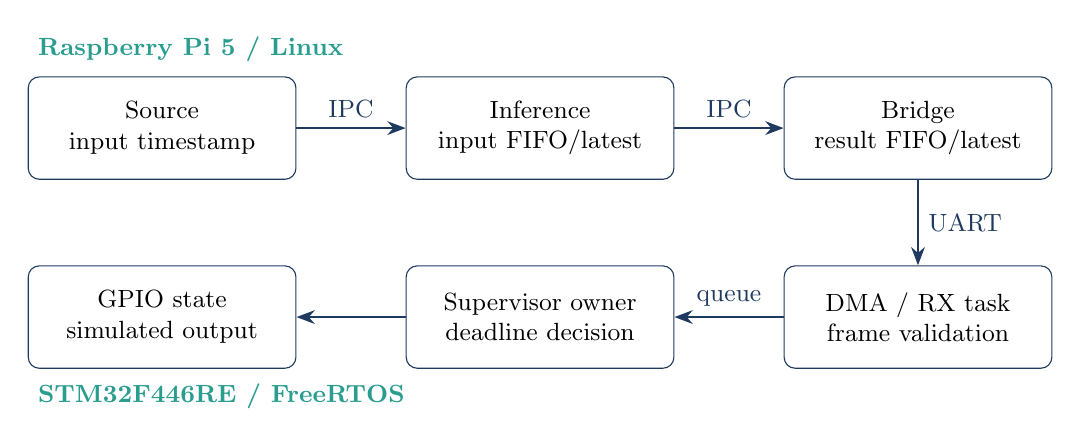
\begin{tikzpicture}[box/.style={draw=navy,rounded corners,align=center,minimum width=34mm,minimum height=13mm,font=\small},arr/.style={-{Stealth},thick,navy}]
\node[box] (s) at (0,0) {Source\\input timestamp};
\node[box] (i) at (4.8,0) {Inference\\input FIFO/latest};
\node[box] (b) at (9.6,0) {Bridge\\result FIFO/latest};
\node[box] (r) at (9.6,-2.4) {DMA / RX task\\frame validation};
\node[box] (v) at (4.8,-2.4) {Supervisor owner\\deadline decision};
\node[box] (o) at (0,-2.4) {GPIO state\\simulated output};
\draw[arr] (s)--node[above,font=\small]{IPC}(i);
\draw[arr] (i)--node[above,font=\small]{IPC}(b);
\draw[arr] (b)--node[right,font=\small]{UART}(r);
\draw[arr] (r)--node[above,font=\small]{queue}(v);
\draw[arr] (v)--(o);
\node[anchor=west,text=teal,font=\small\bfseries] at (-1.7,1) {Raspberry Pi 5 / Linux};
\node[anchor=west,text=teal,font=\small\bfseries] at (-1.7,-3.4) {STM32F446RE / FreeRTOS};
\end{tikzpicture}
\caption{Implemented forward path and ownership; IPC uses Unix datagrams. MCU status and echo replies return over the full-duplex UART.}\label{fig:architecture}
\end{figure}
The split makes several delays independently observable. Source-to-completion time includes input waiting and preprocessing; completion-to-send includes outbound IPC and bridge residence; send-to-receive includes software and transport effects. Preserving the original input timestamp prevents a recent completion timestamp from hiding old input.

Bounded memory does not imply bounded age. A FIFO may preserve increasingly stale work until it fills. Latest-value replacement trades completeness for recency at its particular boundary. Both policies are exposed as experiment settings, with replacement, skipping, missing delivery and queue drop counted separately.
\subsection{Wire format and version evolution}
Each frame contains a two-byte start marker, version, type, 16-bit sequence, one-byte length, payload, and CRC-16/CCITT-FALSE. Payload length is bounded at 64 bytes. CRC covers version through payload; the frame overhead is nine bytes. A sequence gap is evidence of discontinuity, not an authenticated explanation of its cause.

Protocol v1 inference carries input and completion timestamps, input sequence, class and confidence. Protocol v2 appends a 32-bit age-at-send duration. Legacy age is absent, not measured zero. The current encoder emits v3, which retains v2 inference semantics and adds heartbeat session identity and optional diagnostics. Wire versions are independent of the v1/v2 \emph{analysis validity rules} discussed later.
\src{protocol/PROTOCOL.md; linux/README.md}
\page
\subsection{Supervisor state and restart contract}
The supervisor starts in INIT, where output is suppressed. Accepted live heartbeat and fresh result information permit FRESH. Result source-age expiry causes HOLD, and further expiry causes latched FAILSAFE. Heartbeat timeout can enter FAILSAFE directly. Table~\ref{tab:state} gives the concrete indicator semantics.
\begin{table}[H]\centering
\caption{Configured state outputs; these are design semantics, not actuator validation.}\label{tab:state}
\begin{tabular}{llll}\toprule State & PA5 & PB5 & Meaning\\\midrule
INIT & 0 & 0 & Await usable traffic\\FRESH & 1 & 1 & Simulated fresh output enabled\\HOLD & 0 & 1 & Fresh output inhibited\\FAILSAFE & 0 & 0 & Latched fallback\\\bottomrule\end{tabular}
\end{table}
The retained experiment configuration uses provisional heartbeat timeout 100 ms, source-age HOLD 200 ms, source-age FAILSAFE 500 ms, and a 5 ms transit allowance. The portable core's healthy-rearm interval is 1000 ms; the board port exposes no remote or automatic rearm, so a new physical test uses reset. These values are ASSUMED configuration, not calibrated safety limits. The captured E4 threshold snapshot is empty/null; source constants must not be presented as a populated runtime snapshot.

Source age is estimated as
\begin{equation}
 A_{\mathrm{source}}=A_{\mathrm{send}}+(t_{\mathrm{now,MCU}}-t_{\mathrm{rx,MCU}})+B_{\mathrm{transit}}.
\end{equation}
The age-at-send term is a Pi duration. The elapsed receipt term is MCU-local. The allowance is provisional and does not turn serialization arithmetic into an end-to-end bound. The legacy receipt-silence policy cannot recover an absent source-age term.

Expiry is checked before arrivals, preventing late traffic from erasing a deadline violation. Duplicate and old events do not renew freshness. A v3 heartbeat session identifies a bridge incarnation; changing it resets sequence and healthy-history state without bypassing a latched FAILSAFE. A separate local generation stamp invalidates already queued events after session change or rearm. It is not transmitted and must remain attached to the original handoff.
\subsection{Clock alignment}
The shared clock helper filters echo samples and fits an affine offset with drift, reporting residual RMS. The 32-bit microsecond timer is extended chronologically; gaps at or above half-range are ambiguous. Mapping is analytical, not a change to either clock. DMA receipt means the RX task reads the final CRC byte, while transmit time is sampled before response encoding and transmission. Neither is a physical pin timestamp. Consequently, mapping uncertainty remains separate from the supervisor's local reason-based intervals.
\src{stm32/src/supervisor.c; protocol/CLOCK_SYNC.md}
\page
\section{Implementation}
\subsection{Linux modules and execution model}
The Linux path uses separate source, inference, bridge and receiver processes. The C bridge's event loop multiplexes IPC and nonblocking serial traffic; the design does not add a bridge thread for each responsibility. The inference process can create ONNX Runtime workers, so its thread count and actual placement are separate from the process layout.
\begin{table}[H]\centering\small
\caption{Implementation modules and responsibilities.}\label{tab:modules}
\begin{tabularx}{\linewidth}{lX}\toprule Module & Responsibility\\\midrule
\path{linux/src/hea_source.c} & Periodic input identities and timestamps\\
\path{linux/inference/infer_server.py} & Workload, FIFO/latest input selection, skips\\
\path{linux/src/hea_bridge.c} & Result queue, heartbeat, UART and echo logging\\
\path{linux/src/hea_rx.c} & Software receiver and timing records\\
\path{linux/src/hea_runtime.c} & Applied scheduling, affinity and clock helpers\\
\path{protocol/src/hea_proto.c} & Shared encoding, parsing and integrity checks\\
\path{stm32/src/supervisor.c} & Portable deadline/state policy\\
\path{stm32/firmware/main.c} & Tasks, board I/O, timer and diagnostics\\\bottomrule\end{tabularx}
\end{table}
The bridge FIFO is a bounded 256-record queue; latest mode replaces unsent inference. Heartbeats receive priority between frames. A partially submitted frame is immutable: it completes within the 2 ms submission budget or is abandoned by flushing queued output, counting \texttt{expired}, advancing the sequence and waiting a quiet interval. This bounds submission delay and accounts for loss; it describes current software, not verified behavior in historical acquisitions. The age-at-send field is formed at the software-send boundary, covering upstream age and bridge waiting while excluding subsequent kernel/TTY and physical transport delay.

Linux timestamps use \texttt{CLOCK\_MONOTONIC\_RAW}. Periodic sleeping uses the supported monotonic sleep mechanism; the two roles must not be confused in logs. The macOS host checks use a documented clock fallback and cannot validate Linux scheduler behavior.
\subsection{Applied scheduling configuration}
In the retained software P1 campaign, source and bridge use FIFO priorities 60 and 70 on CPU 1 with memory locked; inference uses ordinary scheduling on CPU 0. These recorded settings supersede the earlier guide's illustrative bridge priority 50. Cyclictest P1 is a different experiment: its measured thread uses FIFO 50 on CPU 0.

The nominal source and heartbeat periods are 100 ms and 20 ms. A requested period is not a guarantee during a stall. CPU stress is placed on CPUs 2--3; stream/cache stress uses CPU 2. This placement helps expose shared-resource effects beyond direct contention for the inference CPU. Quota benefits and a packaged real-time-kernel P3 comparison remain PLANNED, not measured.
\page
\subsection{Firmware tasks, interrupts and DMA}
The firmware statically creates supervisor, RX and status/TX tasks at priorities 3, 2 and 1. The supervisor is the sole state-machine writer. Frame and echo queues each have eight slots; transition events use a separate static ring. Overflow is counted and must not refresh a deadline. UART transmission remains outside the supervisor's critical decision path.

The default USART1 receive path uses a 2048-byte circular DMA ring with idle notification and periodic polling. At nominal 921600 baud and 8N1, the ring holds approximately $2048 \times 10 / 921600 = 0.022222\ldots$ s, or 22.22 ms of continuous line traffic. This is CALCULATED capacity, not a lossless-service guarantee. A potential unseen full lap or receive discontinuity causes conservative parser handling. The IRQ alternative retains timestamped byte records and requires the CPU to service incoming bytes promptly.

A regression investigation localized excessive interrupt masking around supervisor calls as a plausible receive hazard. Removing broad masks and moving to DMA addresses that hazard, but the historical A/B counters alone do not prove a unique physical root cause. Final code-review fixes were compiled; they have \textbf{not been flashed or verified on the rig}. Earlier retained runs describe earlier firmware behavior and must not be used to certify the final image.

The nominal board configuration uses ST-LINK MCO as an 8 MHz HSE bypass source, an 84 MHz core, a 1 MHz TIM2 counter, and a 1 kHz FreeRTOS tick. HSI startup fallback is diagnosed. A relative SysTick/TIM2 check can expose disagreement between those clocks' configured rates; it cannot detect a shared oscillator error.
\subsection{Tools and reproducibility}
The host workstation provides editing, portable tests, cross-compilation and report generation. Linux applications and experiment runners execute on the Pi. Firmware executes on the STM32. Keeping these environments explicit prevents a passing macOS test from being mistaken for a target scheduling result.

\path{tools/timing/} runs the wake-up diagnostic; \path{tools/experiments/} records campaigns and settings; \path{analysis/} computes latency, age and fault summaries; \path{tools/la/} supports independent analyzer captures. The retained data include failures and exclusions. This report's own generator reads those files and emits tables plus SHA-256 source hashes without changing the measurement record.

Build configuration is part of provenance. Earlier rapid profile switching could reuse objects because of coarse timestamps; the firmware build now forces recompilation after configuration changes. A successful build establishes interface and link consistency, not stack margin, DMA arbitration behavior, electrical timing, or a worst-case deadline.
\src{stm32/firmware/README.md; tools/experiments/README.md}
\page
\section{Evaluation method}
\subsection{Rig, profiles and loads}
The retained platform is a Raspberry Pi 5 with 4 GB RAM running stock Ubuntu kernel \texttt{6.8.0-1064-raspi} (PREEMPT\_DYNAMIC), connected to an STM32F446RE Nucleo. The physical UART configuration uses Pi GPIO14/15 and MCU USART1 PA10/PA9, common ground and 3.3 V signaling at nominal 921600 baud. The actual Pi device node must be verified from provisioning rather than inferred from these pin names.

The supply is recorded as 5 V / 3 A; the inference baseline reports 4.66--4.92 V under load. Power contamination is therefore a measured experimental limitation. A Pi wall clock approximately three days behind explains inner acquisition timestamps; same-clock monotonic durations remain meaningful.

The experiment families deliberately measure different paths. Cyclictest observes wake-up behavior, inference-only tests observe synchronous model calls, E1--E3 observe a software pipeline over a pseudo-terminal (PTY), and E4/F5 observe physical MCU decisions. Real-UART E3 adds a physical receive endpoint but has no accepted runs. These endpoints cannot be substituted for one another.
\begin{table}[H]\centering\small
\caption{Exposure and acceptance under stored rules; counts refer to runs or attempts.}\label{tab:exposure}
\begin{tabularx}{\linewidth}{lXl}\toprule Set & Exposure / scope & Accepted\\\midrule
Cyclictest & Three 120 s repeats per profile/load & 30/30\\
Inference & 1000 timed calls after 50 warm-ups per run & 21/24\\
E1 / E2 / E3 & Three repeats per cell; nominal 60 s, PTY & 45/45\\
E3b & Input policy comparison; all loaded runs invalid & 3/12\\
Real-UART E3 (original U) & Three repeats in six cells & 0/18\\
Real-UART rerun (U2) & Separate diagnostic attempts; all FLAGGED & 0/18\\
Original E4 & F1--F4 performed; five F5 entries unperformed & 17/25\\
Extra F4 & Short-window transitions; three startup failures & 5/9\\
Separate F5 & Short-window stale-result transitions & 5/5\\\bottomrule\end{tabularx}
\end{table}
The timer and software campaigns use the performance governor; the inference baseline uses ondemand and affinity CPUs 0--3. This difference precludes a controlled direct comparison between inference-call and pipeline numbers. Most comparison cells have three repeats, below the planned five-valid-repeat gate. Repetition counts and exclusion reasons accompany each interpretation instead of being hidden by pooled samples.
\src{results/README.md; docs/STAGE_REPORT.md}
\page
\subsection{Metrics, denominators and validity versions}
For Pi timestamps, service latency is input-to-inference completion and delivery latency is input-to-reception. Service includes input waiting and preprocessing; it is not the model call alone. In aggregate latency tables, P50/P99 values are medians of per-run quantiles, while maxima are the largest observed per-run maxima. E3b and real-UART E3 tables instead report each run separately. A maximum over finite exposure is not a worst-case bound.

Held-value AoI integrates the rising age between informative updates. For a segment starting at age $d$ and lasting $h$, its area is $dh+h^2/2$. E3 includes stalls and the final tail within the declared RAW-clock measurement window, excluding shutdown drain, but age is undefined before the first informative delivery. The mean uses initialized time. Violation time above threshold $\tau$ is time-weighted; reception deadline misses count CRC-valid receptions above strict 100/150 ms thresholds, including shutdown drain. Missing inputs remain separate and are not silently added to this reception denominator.

Fault timing uses three conceptual events: onset, MCU decision and physical output. A mapped onset-to-decision interval relies on echo alignment. A local interval instead starts at the last accepted heartbeat or inference, selected by the transition reason. Reason 3 denotes heartbeat timeout; reasons 9/10 denote source-age HOLD/FAILSAFE. Mixing those reference events produces a misleading distribution even if every subtraction is numerically correct.

\textbf{MEASURED} identifies recorded observations within the stated acceptance scope. \textbf{FLAGGED} identifies observations from invalid or unqualified runs. \textbf{PLANNED} identifies unperformed work; \textbf{UNKNOWN} identifies missing evidence. CALCULATED, ASSUMED and INFERRED are used only to distinguish arithmetic, configured choices and explanations, following the stage report.

Stored validity v1 requires the campaign's recorded process/settings evidence and power checks. For software campaigns, pre-existing sticky bits alone do not exclude a run; live bits or newly set sticky bits do. The earlier smoke exclusions retain their original rule rather than being retrospectively promoted.

The final v2 review requires RAW-timestamped monitor coverage of the full window with gaps at most 1.5 s, stressor liveness during measurement, and clock fits no older than 5 s. Read-only replay confirms 0/45 older E1--E3 runs under v2 because the monitor lacks RAW timestamps; cyclictest retains 3/15 per profile because stressed runs lack liveness records. E4 remains 17/25, and analyzer numbers/flags are unchanged. These are missing-evidence limits, not detected faults in the v1 observations. New acquisitions must use v2.
\page
\section{Results}
\subsection{Timer wake-up and inference-only behavior}
Table~\ref{tab:timer} shows smaller FIFO wake-up tails across the five loads. Under idle conditions P1 P99 is 9 $\mu$s; under memrate it reaches 239 $\mu$s. The observation supports the scheduling benefit while showing that real-time priority does not remove interference from other cores. The ordinary-policy median includes the default timer-slack effect, so its gap from FIFO cannot be attributed entirely to scheduler waiting.
\begin{table}[H]
\centering\small
\caption{MEASURED under v1: timer wake-up latency ($\mu$s), three repeats per cell.}\label{tab:timer}
\begin{tabular}{lrrrr}
\toprule
Load & P0 P99 & P0 max & P1 P99 & P1 max \\
\midrule
idle & 57 & 2659 & 9 & 92 \\
cpu c2,3 & 68 & 2636 & 11 & 73 \\
stream c2 & 300 & 3565 & 39 & 211 \\
cache 2M c2 & 203 & 4780 & 35 & 233 \\
memrate c2,3 & 613 & 5170 & 239 & 1094 \\
\bottomrule
\end{tabular}
\end{table}

These are MEASURED v1 wake-up observations from three 120 s repeats per cell. Stressed runs lack the liveness evidence required by v2. They measure neither UART delay nor inference latency.

Table~\ref{tab:infer} shows that adding inference threads is not consistently beneficial. Idle P50 improves from one to three threads, while under CPU stress the four-thread P50 and tail are worse than the one-thread case. Different valid repeat counts limit confidence in the four-thread cells.
\begin{table}[H]
\centering\small
\caption{MEASURED accepted subset: inference-call latency (ms).}\label{tab:infer}
\begin{tabular}{lrrrrr}
\toprule
Load & Threads & Valid & P50 & P99 & Max \\
\midrule
idle & 1 & 3 & 44.0 & 48.0 & 57.0 \\
idle & 2 & 3 & 31.1 & 42.9 & 51.8 \\
idle & 3 & 3 & 29.4 & 38.5 & 52.8 \\
idle & 4 & 1 & 31.4 & 70.7 & 94.1 \\
cpu stress c2,3 & 1 & 3 & 45.1 & 53.7 & 65.5 \\
cpu stress c2,3 & 2 & 3 & 33.2 & 46.1 & 105.5 \\
cpu stress c2,3 & 3 & 3 & 45.5 & 77.6 & 91.1 \\
cpu stress c2,3 & 4 & 2 & 60.3 & 100.5 & 150.3 \\
\bottomrule
\end{tabular}
\end{table}

The model is \texttt{mobilenetv2-12.onnx}, with recorded ONNX Runtime 1.31.0. Preprocessing P50 is approximately 2.4 ms and is separate from the call timings. The three excluded runs have live under-voltage. No missing P95 or cold-start statistic is reconstructed from the available quantiles.
\page
\subsection{E1 contention and E2 runtime tuning}
Table~\ref{tab:e1} reports the E1 software endpoint. CPU-only load on other cores produces a much smaller change than memrate. Under memrate, service and delivery grow into seconds while their difference remains small relative to the accumulated age. This suggests that the dominant delay occurs before transport to the software receiver, rather than being a slow UART effect: this experiment does not use a physical UART.
\begin{table}[H]
\centering\small
\caption{MEASURED under v1: E1 P0 software/PTY latency (ms); three repeats.}\label{tab:e1}
\begin{tabular}{lrr}
\toprule
Load & Service P50/P99/max & Delivery P50/P99/max \\
\midrule
Idle & 44.25/48.28/56.31 ms & 44.37/48.47/56.47 ms \\
Stream & 76.46/88.5/202.8 ms & 76.99/89.02/203.4 ms \\
Memrate & 6626/13980/15120 ms & 6626/13980/15120 ms \\
Cache 2M & 67.58/97.3/121.6 ms & 68/98.83/121.8 ms \\
CPU & 45.2/48.13/80.74 ms & 45.41/48.3/80.98 ms \\
\bottomrule
\end{tabular}
\end{table}

Table~\ref{tab:e2} compares the recorded P0 and P1 configurations. The memrate median is somewhat lower under P1, but the largest observed service maximum remains large and is higher in the P1 cell. Cache-loaded tails also do not show a uniform improvement. The data support a limited conclusion: priority and placement are useful controls, but they do not solve this pipeline's overload.
\begin{table}[H]
\centering\small
\caption{MEASURED under v1: E2 software/PTY latency (ms); three repeats.}\label{tab:e2}
\begin{tabular}{lrr}
\toprule
Profile/load & Service P50/P99/max & Delivery P50/P99/max \\
\midrule
P0 / idle & 43.9/49.15/58.33 ms & 44.02/49.29/58.51 ms \\
P0 / memrate & 6506/13260/13410 ms & 6506/13260/13410 ms \\
P0 / cache & 66.36/73.1/108.8 ms & 66.81/73.57/109.6 ms \\
P1 / idle & 43.94/48.81/56.24 ms & 44.07/48.98/56.41 ms \\
P1 / memrate & 6000/12890/14070 ms & 6002/12890/14070 ms \\
P1 / cache & 69.8/96.58/135.7 ms & 70.19/97.16/136.1 ms \\
\bottomrule
\end{tabular}
\end{table}

All rows are MEASURED under v1, with three valid repeats per cell. They are not confirmed by the stricter v2 coverage replay. The summaries retain zero reported queue drops for these rows, but zero bridge drops cannot establish that inputs avoided waiting elsewhere. A queue that grows without overflowing during the observation period can already produce unacceptable freshness.

The contrast between this table and inference-only timing is instructive. A multi-second service interval need not mean a single model invocation consumed seconds of CPU time. Service starts at input generation, before queued waiting. Disaggregating stage timestamps is therefore essential to answer RQ1 without confusing scheduler behavior, computation demand and queue residence.
\src{results/2026-10-11_e1_e2_e3_pty/20261008T103412Z_e_onnx/summary/README.md}
\page
\subsection{E3: bridge replacement and upstream backlog}
Table~\ref{tab:e3} compares bridge FIFO and latest policies while preserving the software endpoint. Under idle load their age statistics are close. Under memrate both retain multi-second mean age and both report zero bridge replacements. A replacement slot cannot discard work that has not yet reached that slot.
\begin{table}[H]
\centering\small
\caption{MEASURED under v1: E3 held-value AoI and median per-run counts.}\label{tab:e3}
\begin{tabular}{lrrrr}
\toprule
Load/policy & Mean age (ms) & Peak (ms) & Received & Replaced \\
\midrule
Idle/fifo & 94.69 & 158 & 602 & 0 \\
Idle/latest & 94.59 & 156 & 602 & 0 \\
Memrate/fifo & 6660 & 13660 & 480 & 0 \\
Memrate/latest & 6958 & 14170 & 472 & 0 \\
\bottomrule
\end{tabular}
\end{table}

\begin{table}[H]
\centering\small
\caption{MEASURED under v1: E3 strict-threshold outcomes; medians per run over three repeats. Miss denominators count CRC-valid inference receptions including drain.}\label{tab:e3_thresholds}
\begin{tabular}{lrrr}
\toprule
Load/policy & Time $>$100 ms (s) & Time $>$150 ms (s) & Misses $>$100/$>$150 ms \\
\midrule
Idle/fifo & 26.85 & 0.0104 & 0/0 of 602 \\
Idle/latest & 26.79 & 0.001595 & 0/0 of 602 \\
Memrate/fifo & 60.23 & 60.23 & 480/480 of 480 \\
Memrate/latest & 60.24 & 60.24 & 472/472 of 472 \\
\bottomrule
\end{tabular}
\end{table}

The retained source period is 100 ms. Loaded median completion intervals are approximately 122--130 ms across these runs. The resulting evidence supports an upstream backlog explanation: inputs arrive faster than the loaded inference stage completes them. A newly completed inference can therefore be an old input, even if the bridge forwards it immediately.

E3's mean uses initialized time, while peak age is the largest observed peak. Median per-run generated counts are 602 idle and 605 loaded. Loaded FIFO delivers 480, with 125 missing; latest delivers 472, with 132 missing. These medians are not pooled totals. Table~\ref{tab:e3_thresholds} shows about 60.2 s above each threshold under load. At idle, FIFO/latest spend 26.85/26.79 s above 100 ms despite zero reception misses at either threshold (602 receptions per run, median). Age rises between deliveries, so timely receptions do not ensure continuously fresh held values. Even idle time above 150 ms is nonzero. These are per-run medians over initialized measurement time; endpoint windows explain deviations from the nominal 60 s source duration.

\page
\subsection{E3b: input replacement under power contamination}
The E3b change moves replacement before the expensive computation. It drains available source datagrams and selects the latest valid input before invoking inference; superseded inputs are logged as \texttt{skipped\_stale}. Table~\ref{tab:e3b} is regenerated from raw reception and inference CSVs.
\begin{table}[H]
\centering\small
\caption{FLAGGED: all six loaded E3b runs fail live-power validity. Per-run input-to-software-reception age $(t_{rx,ns}-t_{input,ns})/10^6$ (ms); nearest-rank quantiles over CRC-valid inference receptions including shutdown drain.}\label{tab:e3b}
\begin{tabular}{lrrrr}
\toprule
Input/repeat & Receptions & P50 (ms) & P99 (ms) & Skipped \\
\midrule
fifo/r1 & 455 & 8676.0 & 15891.0 & 0 \\
fifo/r2 & 475 & 6527.4 & 13821.6 & 0 \\
fifo/r3 & 457 & 7193.5 & 15579.1 & 0 \\
latest/r1 & 435 & 189.3 & 254.0 & 171 \\
latest/r2 & 435 & 190.3 & 256.0 & 172 \\
latest/r3 & 432 & 190.7 & 267.9 & 173 \\
\bottomrule
\end{tabular}
\end{table}

Every loaded E3b row is FLAGGED for live power/throttle events. The large difference supports a diagnostic mechanism to test, but cannot establish a clean causal improvement. Only three idle runs are accepted across the whole E3b campaign, and their policy counts are unequal. RQ2 therefore has an architectural explanation and an implemented remedy, with clean loaded validation still UNKNOWN.
\page
\subsection{Real-UART E3: diagnostic evidence only}
The original real-link campaign (U in Appendix A) retains 18 runs, of which none is valid. The following table and observations refer only to U. Live power/throttle bits occur in 16, all nine memrate runs fail the 200 $\mu$s clock-fit RMS gate, and 14 lack transition events. These overlapping reasons must not be summed as disjoint exclusions. Table~\ref{tab:real} reports MCU-computed source-age quantiles from the loaded raw records, including drain.
\begin{table}[H]
\centering\small
\caption{FLAGGED: loaded real-UART E3 MCU source-age estimates.}\label{tab:real}
\begin{tabular}{lrrr}
\toprule
Input/bridge/repeat & Receptions & P50 (ms) & P99 (ms) \\
\midrule
fifo/fifo/r1 & 433 & 9412.861 & 17995.587 \\
fifo/fifo/r2 & 447 & 8900.786 & 16784.222 \\
fifo/fifo/r3 & 440 & 9405.502 & 17389.963 \\
fifo/latest/r1 & 429 & 9380.214 & 18520.423 \\
fifo/latest/r2 & 439 & 8638.846 & 17483.123 \\
fifo/latest/r3 & 428 & 9207.069 & 18588.409 \\
latest/latest/r1 & 449 & 189.510 & 253.305 \\
latest/latest/r2 & 476 & 183.432 & 260.011 \\
latest/latest/r3 & 427 & 196.503 & 254.537 \\
\bottomrule
\end{tabular}
\end{table}

The physical endpoint reproduces the qualitative backlog pattern: input FIFO is associated with seconds of age even when the bridge uses latest replacement; input-latest reception ages lie near the provisional 200 ms HOLD threshold. This is a FLAGGED observation, not a valid physical policy comparison. MCU age includes the provisional transit allowance and is distinct from mapped receipt age, which also depends on the echo fit.

All three loaded latest/latest event files are empty and all their reception states are FAILSAFE. The fractions of reception ages above 200 ms are 40.5\%, 32.8\%, and 45.2\% in the stage report. They are \emph{not} HOLD occupancy or transition rates. A latched FAILSAFE does not leave that state merely because a subsequent result is less old.

An empty transition log is not generally evidence of bad freshness: a continuously FRESH system could have no new transitions. The runner's empty-event rejection is therefore a validity-rule limitation. In these particular captures, however, the reception states do not support assuming FRESH. No missing state history is invented to fill the gap.

The retained idle observations have MCU age near 53 ms, but they too remain FLAGGED within this campaign. One idle run includes negative mapped-age samples, and the original quantiles preserve them. Excluding anomalous samples without a declared rule would conceal the clock/observation problem rather than resolve it.

\textbf{Separate FLAGGED rerun (U2).} The later \texttt{20261012T160628Z} campaign retains 18 further attempts, 0 accepted: all 18 have live-power exclusions and 6 also have pipeline failures. Its diagnostic ages and state durations are excluded from the comparison presented here and are not pooled with U. They do not validate HOLD occupancy under clean conditions. Appendix A identifies the retained summaries.

\page
\subsection{E4 and F5: reason-based physical state timing}
Table~\ref{tab:e4} recomputes local intervals from raw STATE\_EVENT records for the original accepted E4 runs. F1 kills the bridge; F2 stops it; F3 stops inference; F4 runs a FIFO-99 CPU hog. HOLD reason 9 uses the last accepted inference, whereas heartbeat FAILSAFE reason 3 uses the last heartbeat. The columns therefore have explicitly different origins.
\begin{table}[H]
\centering\small
\caption{MEASURED: original E4 reason-based MCU-local intervals (ms).}\label{tab:e4}
\begin{tabular}{lrrrr}
\toprule
Fault & Valid & HOLD P50/max & FAILSAFE P50/max & Safe ref. \\
\midrule
F1 & 5 & 175.317 / 175.535 & 100.456 / 100.641 & HB \\
F2 & 5 & 175.206 / 175.709 & 100.577 / 100.596 & HB \\
F3 & 5 & 175.754 / 175.815 & 475.754 / 475.815 & Result \\
F4 & 2 & --- & 100.639 / 100.931 & HB \\
\bottomrule
\end{tabular}
\end{table}

F1/F2 heartbeat FAILSAFE spans 100.128--100.641 ms. Their earlier HOLD appears about 175 ms after inference, consistent with a 200 ms source-age threshold after including send age and transit allowance. Its roughly 98 ms heartbeat age is not an early heartbeat timeout. The observed timing does not establish a tick-rate fault.

Table~\ref{tab:f5} isolates freshness from liveness. SIGUSR1 suppresses inference results while the bridge continues heartbeat traffic. At HOLD, the latest heartbeat is only approximately 17--19 ms old. The supervisor nevertheless rejects stale information, then enters source-age FAILSAFE.
\begin{table}[H]
\centering\small
\caption{MEASURED: F5 short-window transitions (ms), five accepted runs.}\label{tab:f5}
\begin{tabular}{lrrr}
\toprule
Repeat & Result to HOLD & HB age at HOLD & Result to FAILSAFE \\
\midrule
r1 & 175.917 & 18.462 & 475.917 \\
r2 & 175.343 & 18.510 & 475.343 \\
r3 & 174.950 & 17.459 & 474.950 \\
r4 & 175.596 & 18.336 & 475.596 \\
r5 & 175.767 & 18.494 & 475.767 \\
\bottomrule
\end{tabular}
\end{table}

F5 is MEASURED for five accepted short-window runs. The 175/475 ms receipt-relative intervals do not redefine the configured 200/500 ms source-age thresholds. The internal SysTick/TIM2 check reports $-8$ ppm over a 1000 ms window in F5 r5; independent absolute clock calibration remains UNKNOWN.

Five of nine extra F4 attempts pass short-window transition checks, in addition to the original two of five. Three extra attempts fail startup and one exceeds the RMS gate. The combined seven of fourteen accepted F4 attempts do not share equal exposure/recovery scope. Their heartbeat FAILSAFE spans 100.405--100.931 ms. Six enter FAILSAFE directly; one first enters source-age HOLD. Pooling first-transition intervals would mix reference events.
\page
\subsection{Bring-up and independent-capture limitations}
The bring-up series is diagnostic evidence, not a clean latency campaign. Table~\ref{tab:smoke} includes the seventh retained smoke in addition to the first six discussed by the stage report. All are excluded by their original summaries.
\begin{table}[H]
\centering\small
\caption{FLAGGED: all seven bring-up summaries exclude their runs.}\label{tab:smoke}
\begin{tabular}{lr}
\toprule
Retained smoke & Timing qualification \\
\midrule
hw\_smoke1 & FLAGGED \\
hw\_smoke2 & FLAGGED \\
hw\_smoke3\_hsi & FLAGGED \\
hw\_smoke4\_batt & FLAGGED \\
hw\_smoke5\_oldfw & FLAGGED \\
hw\_smoke6\_dma & FLAGGED \\
hw\_smoke7\_infrx & FLAGGED \\
\bottomrule
\end{tabular}
\end{table}

The stage report records an HSI echo-fit drift of 18839.975 ppm and RMS 1083.883 $\mu$s in smoke1, compared with 89.040 ppm and 39.581 $\mu$s for the final smoke6 fit. These FLAGGED observations motivated clock investigation; echo drift is not direct UART bit timing. Smoke6's retained status reports zero UART/CRC errors and zero split error/drop/event-loss counters, but one excluded finite run cannot prove lossless reception.

The repository also retains analyzer captures acquired after the original fault section was written. Table~\ref{tab:analyzer} inventories their summary rows. The collection remains FLAGGED: F1-r05 is incomplete, generated comparisons retain hardware-qualification warnings, and MCU/analyzer intervals can use different reference events.
\begin{table}[H]
\centering\small
\caption{FLAGGED: retained analyzer summary inventory; rows are not acceptance counts.}\label{tab:analyzer}
\begin{tabular}{lrr}
\toprule
Collection & Summary rows & Status \\
\midrule
run\_F1 & 4 & FLAGGED \\
run\_F2 & 5 & FLAGGED \\
run\_F4 & 5 & FLAGGED \\
check\_F2 & 1 & FLAGGED \\
\bottomrule
\end{tabular}
\end{table}

The analyzer observes physical edges and estimated UART byte ends; MCU events refer to accepted protocol messages. Subtracting these intervals does not automatically measure clock error because the reference packet and observation boundary can differ. A nominal 24 MHz sample clock gives a sample interval, not a calibration certificate.

These captures are retained as evidence to qualify, not promoted into an output-latency bound. The report therefore distinguishes the measured MCU state decision from independently qualified physical output activation. For RQ3, the former has accepted examples; the latter remains incomplete.
\page
\section{Discussion and limitations}
\subsection{What the results explain}
The experiments connect three OS mechanisms. First, latency remains elevated under cross-core memrate stress despite the P1 configuration (MEASURED under v1). Shared-memory interference is an INFERRED explanation, not a causally isolated finding. Second, IPC and queue policy determine which input is processed, so freshness can deteriorate while every completed result is promptly transmitted. Third, independent supervision separates communication liveness from the usefulness of the communicated value.

The negative bridge-replacement result is particularly useful. It prevents an attractive but incorrect generalization that a one-slot output buffer guarantees fresh information. Replacement must address the accumulating boundary, and even correctly placed replacement cannot bound a computation that can stall indefinitely. A physical observer strengthens the architecture, but its own logs and clock mapping require validation.

The reason-based E4 correction similarly demonstrates why semantic review must accompany statistics. Selecting the first departure from FRESH and assigning its reference from the injected fault produced a plausible number with the wrong meaning. Using the transition reason restores the correspondence between the state-machine condition, the clock reference, and the configured threshold.
\subsection{Threats to validity and transfer}
Power is the largest identified obstacle to clean loaded comparisons. Sampled flags can miss disturbances between observations, and accepted runs under the recorded rule are not proof of perfect electrical conditions. Unequal repetitions, short exposure, different governors and non-identical observation windows limit cross-campaign conclusions. No statistical confidence interval or rare-event bound is claimed from three-repeat cells.

Software PTY experiments exclude physical serialization and MCU scheduling. Real-UART age observations are all FLAGGED. MCU-local timestamps avoid cross-clock subtraction for silence intervals, but their absolute rate and GPIO correspondence still require independent qualification. Clock-fit residuals are not deterministic error bounds; the fault being studied can also starve the bridge's echo observer.

The final firmware fixes are compiled but not flashed/rig-verified. Static RAM/link sizes do not establish stack high-water margins. DMA finite-capacity handling is not proof of unrestricted losslessness. The system includes neither a physical actuator nor an independent MCU hardware watchdog.

Transfer to a balancing robot is PLANNED. The reusable elements are stage timestamps, queue placement, applied-setting records and fault methodology. Thresholds, pins, workload timing and safe-state semantics must be re-established on the destination rig. In particular, suppressing a Pi proposal may need to preserve local balancing control; copying this demonstration's low GPIO output as ``stop everything'' would not be justified.
\page
\section{Conclusion and future work}
This course project demonstrates a heterogeneous OS experiment architecture in which Linux performs variable computation and a separate FreeRTOS controller evaluates liveness and freshness. Its value lies in making processor scheduling, cross-core interference, buffering and independent deadlines observable within one reproducible pipeline.

RQ1 is answered within the retained v1 measurement scope: FIFO substantially improves wake-up tails, but memory contention continues to increase latency. Inference threading has workload-dependent effects, and pipeline service includes waiting that a model-call benchmark excludes. The stricter v2 replay cannot confirm older stressed/software runs because additional evidence was not recorded; their v1 labels remain explicit.

RQ2 identifies the replacement boundary as decisive. Bridge latest-value replacement leaves upstream queued work untouched. Input-latest implementation and flagged reruns support the expected mechanism, but the clean loaded effect remains UNKNOWN. The report does not transform a small buffer into a deterministic age guarantee.

RQ3 is answered for selected physical MCU state transitions. The supervisor responds to heartbeat loss and to stale computation with heartbeat alive. Local timing must follow each transition reason, and mapped onset timing must retain its clock uncertainty. These observations establish neither a worst-case reaction bound nor physical actuator safety.

The next experimental priority is a clean-power, v2-recorded rerun of loaded input-policy and real-UART comparisons, with at least the planned five valid repetitions per cell. The run should preserve failed attempts, startup state, initial age, explicit measurement windows and every skip/drop/loss denominator. Runtime threshold snapshots should be populated rather than inferred later from source.

Independent qualification should capture fault onset, decision and output on a common analyzer clock, reconcile accepted-message versus physical-byte references, and assess absolute oscillator accuracy. Matched IRQ/DMA experiments should retain exact image/configuration identity, UART error counters, queue losses, stack margins and release timing. Final compiled firmware fixes require deployment and hardware testing before any upgraded claim.

Longer stale-result trials should match the steady interval, observation window and recovery protocol. Quota and packaged real-time-kernel profiles remain PLANNED comparisons with matched workload and queue settings. A later robot integration should begin with interface review and shadow logging, then establish its own fallback and rearm semantics. The experiment method transfers; the present timing values and provisional thresholds do not.
\page
\begin{thebibliography}{9}
\bibitem{simplex} S. Bak, D. K. Chivukula, O. Adekunle, M. Sun, M. Caccamo, and L. Sha. ``The System-Level Simplex Architecture for Improved Real-Time Embedded System Safety.'' IEEE RTAS, 2009, pp. 99--107. Full-text verification recorded in \path{docs/research/R1.md}. \url{https://researchconnect.stonybrook.edu/en/publications/the-system-level-simplex-architecture-for-improved-real-time-embe/}
\bibitem{aoi} S. Kaul, R. Yates, and M. Gruteser. ``Status Updates Through Queues.'' CISS, 2012. Full-text verification and applicability limits recorded in \path{docs/research/R2.md}. \url{https://www.winlab.rutgers.edu/~gruteser/papers/Status%20Updates%20Through%20Queues.pdf}
\bibitem{memguard} H. Yun, G. Yao, R. Pellizzoni, M. Caccamo, and L. Sha. ``MemGuard: Memory Bandwidth Reservation System for Efficient Performance Isolation in Multi-core Platforms.'' IEEE RTAS, 2013. Reviewed sections recorded in \path{docs/research/R5.md}. \url{https://www.ittc.ku.edu/~heechul/papers/memguard-rtas13.pdf}
\bibitem{cpufreq} Linux kernel documentation. ``CPU Performance Scaling.'' Reviewed policy/governor sections recorded in \path{docs/research/R4.md}, 6 October 2026. \url{https://docs.kernel.org/admin-guide/pm/cpufreq.html}
\bibitem{sntp} D. Mills. ``Simple Network Time Protocol (SNTP) Version 4 for IPv4, IPv6 and OSI.'' RFC 4330, January 2006, Section 5. Equations reviewed in \path{docs/research/R8.md}. \url{https://datatracker.ietf.org/doc/html/rfc4330#section-5}
\bibitem{r6} Project research note. ``R6 --- Reference architecture review.'' \path{docs/research/R6.md}, 6 October 2026. Pinned implementation review; task-separation concepts only. Submitted task configuration: \path{stm32/firmware/main.c}.
\end{thebibliography}
All external background references above are drawn from sources already reviewed in the repository research notes. No unverified first-pass literature claim is used as a measurement of this rig. Repository evidence paths and exact table-input hashes are given in Appendix A and \path{generated/source-manifest.json}.

Historical plans in the system guides and roadmaps establish intent rather than implementation completion. Where they conflict with retained settings, the recorded settings determine the experimental description. The result inventory also supersedes the stage report's historical statement that no analyzer captures yet existed.
\page
\appendix
\section{Claim-to-evidence traceability}
The reporting checkout is commit \texttt{5e3f461}; its parent cleanup commit \texttt{5575cef} organizes the retained results. These identify the reporting source. The tables below instead give acquisition commits recorded in per-run metadata where available. A recorded Git commit does not prove that a particular MCU binary was flashed; image identity must still be resolved before a hardware rerun. Where no populated firmware/threshold snapshot establishes that identity, it remains UNKNOWN.

For compact raw paths below, define \texttt{R}=\path{results/} and the following acquisition roots. They are literal paths relative to the repository root.
\begin{description}[style=nextline]
\item[C] \path{results/2026-10-11_cyclictest/}
\item[I] \path{results/2026-10-11_inference_baseline/}
\item[E] \path{results/2026-10-11_e1_e2_e3_pty/20261008T103412Z_e_onnx/}
\item[B] \path{results/2026-10-12_e3b_input_latest/20261012T091415Z_e3b/}
\item[U] \path{results/2026-10-12_e3_real_uart/20261012T105039Z_e3real/}
\item[U2] \path{results/2026-10-12_e3_real_uart_rerun/20261012T160628Z_e3real2/}
\item[F] \path{results/2026-10-12_e4_faults/20261012T093526Z_e4/}
\item[S] \path{results/2026-10-12_f5_stale/20261012T101949Z_f5/}
\end{description}
\begin{longtable}{L{.23\linewidth}L{.19\linewidth}L{.45\linewidth}}
\caption{Claims, configuration and raw evidence. Commit column gives acquisition metadata where known.}\label{tab:claims}\\
\toprule Claim / table & Commit / config & Raw run path / summary or figure\\\midrule\endfirsthead
\toprule Claim / table & Commit / config & Raw run path / summary or figure\\\midrule\endhead
FIFO wake-up tails; Table~\ref{tab:timer} & \texttt{9740d1a}; P0 OTHER, P1 FIFO 50 & C/\path{20261008T091937Z_cyc_P0/B0_idle_r1/}; per-run \path{sched_check.txt}, power and histogram records; C/\path{SUMMARY.md}.\\
Thread-count sensitivity; Table~\ref{tab:infer} & \texttt{ad8097d}; ondemand, 1--4 workers & I/\path{idle_r1/threads-1/bench/}; per-run power/validity and \path{SUMMARY.md}.\\
Contention and tuning; Tables~\ref{tab:e1}--\ref{tab:e2} & \texttt{47ae9a9}; P0/P1; applied settings & E/\path{E1_P0_B0_idle_latest_r1/pipeline/}; E/\path{E2_P1_B0_idle_latest_r1/settings.json}; \path{summary/E1_table.csv}, \path{E2_table.csv}.\\
Bridge replacement leaves age; Table~\ref{tab:e3} & \texttt{47ae9a9}; P1, FIFO/latest & E/\path{E3_P1_B2_memrate_c23_fifo_r1/pipeline/}; \path{summary/E3_table.csv}; infer/rx records.\\
\bottomrule
\end{longtable}
\page
\begin{longtable}{L{.23\linewidth}L{.19\linewidth}L{.45\linewidth}}
\caption{Claim-to-evidence table, continued. All flagged scopes remain excluded.}\\
\toprule Claim / table & Commit / config & Raw run path / summary or figure\\\midrule\endfirsthead
\toprule Claim / table & Commit / config & Raw run path / summary or figure\\\midrule\endhead
Input latest diagnostic; Table~\ref{tab:e3b} & \texttt{3a8891a}; input policy; FLAGGED & B/\path{E3B_P1_B2_memrate_c23_latest_r1/pipeline/rx.csv}; sibling \path{infer.csv} and validity.\\
Real-link age; Table~\ref{tab:real} & \texttt{b08e92e}; input/bridge policies; FLAGGED & U/\path{E3_REAL_P1_B2_memrate_c23_input_latest_bridge_latest_r1/pipeline/inf_rx.csv}; per-run conditions, settings, validity.\\
Reason-specific decisions; Table~\ref{tab:e4} & \texttt{fdeaa6f}; original valid E4 subset & F/\path{F2-r01/pipeline/state_events.csv}; F1 uses passive capture records; \path{e4_runs.csv} selects accepted runs only.\\
Freshness despite live heartbeat; Table~\ref{tab:f5} & \texttt{f4ef638}; SIGUSR1, short windows & S/\path{r1/F5-r01/pipeline/state_events.csv}; each repeat's power and \path{run.json}; r5 status for tick check.\\
Extra F4 acceptance & \texttt{f4ef638}, \texttt{b08e92e}; short-window scope & \path{results/2026-10-12_f4_extra/20261012T102112Z_f4/} and \path{20261012T105039Z_f4b/}; per-attempt \path{run.json}, power, echo and events.\\
Bring-up diagnostics; Table~\ref{tab:smoke} & Acquisition UNKNOWN; FLAGGED & \path{results/2026-10-12_hw_bringup/hw_smoke6_dma/}; all seven \path{summary.json}; raw status/echo CSVs.\\
Analyzer qualification incomplete; Table~\ref{tab:analyzer} & Acquisition UNKNOWN; FLAGGED & \path{results/2026-10-12_logic_analyzer/run_F1/}; corresponding F2/F4/check folders, \path{la_e4.csv}, captures.\\
Design ownership; Figure~\ref{fig:architecture} & \texttt{5e3f461}; current source & \path{linux/src/hea_bridge.c}; \path{stm32/firmware/main.c}; no measurement claimed by diagram.\\
\bottomrule
\end{longtable}
\textbf{Later rerun traceability.} U2/\path{summary/per_run.csv} supplies the separate 0/18 acceptance count and exclusions; U2/\path{campaign.json} records P1 settings, three repeats per cell and 921600 baud. Cleanup commit \texttt{5575cef} retains this collection; it is not an acquisition/image identity. U2 is excluded from Table~\ref{tab:real} and all presented policy comparisons.

\textbf{Validity audit.} \path{results/README.md} records the v1/v2 replay counts. \path{docs/STAGE_REPORT.md} supplies the reason-based corrections and extra-F4 acceptance scopes. The generator does not revalidate old runs using today's rules or overwrite historical summaries.

\textbf{Numeric generation.} \path{generate_evidence.py} emits each result table directly from retained CSV or Markdown summaries. E3b, real-UART age, original E4 local intervals and F5 intervals are computed from raw rows. Nearest-rank selection uses $\lceil pn\rceil$; E4 selects the last-event reference by reason. The manifest hashes every table input, allowing a reviewer to detect changed source bytes.
\page
\section{How to reproduce}
\subsection{Build this report on the host}
From the repository root, run:
\begin{verbatim}
python3 submission/report/generate_evidence.py
cd submission/report
latexmk -xelatex -interaction=nonstopmode \
  -halt-on-error main.tex
swift -module-cache-path .swift-cache \
  ../../../../slides/render.swift main.pdf preview
\end{verbatim}
The renderer path points to the main project's shared script; its module cache stays in the report folder. The build requires XeLaTeX/latexmk and Avenir Next/Menlo fonts. The standard-library Python generator writes only \path{submission/report/generated/}. \path{build.sh} performs these steps and records the build log. The review log records visual inspection; regenerated tables and source hashes should match byte-for-byte.

\subsection{Software and target verification commands}
Run these checks from the repository root; after B.1, reset the directory as shown. These commands were \emph{not} rerun as target verification during report production:
\begin{verbatim}
cd ../..  # from submission/report to repository root
make test
make firmware
make -C protocol test-char-modes
make -C stm32 test
python3 -m unittest discover -s analysis/tests -v
\end{verbatim}
Host checks cover portable behavior and synthetic/fake endpoints. Cross-compilation additionally requires the pinned FreeRTOS/CMSIS reference and the Arm toolchain. Do not execute target-only scheduler/device experiments on macOS.

For a new Pi acquisition, use the documented command interfaces and new output directories:
\begin{verbatim}
python3 tools/experiments/e_campaign.py --help
python3 analysis/e_summary.py --help
python3 analysis/e4_summary.py --help
\end{verbatim}
The exact retained campaign invocation is in each run's \path{command.txt}; copy its workload/profile configuration while using new output paths and the current v2 recorder. Verify the actual serial node, supply, applied thread policies and image identity. Firmware flash/reset wrappers and wiring are documented in \path{stm32/firmware/README.md} and \path{scripts/stm32/}. Replaying a report is a read-only host operation; reproducing timing requires the Pi/STM32 rig and a new evidence record.
\page
\section{Mapping to Operating Systems course topics}
\small
\begin{longtable}{L{.22\linewidth}L{.32\linewidth}L{.34\linewidth}}
\caption{OS mechanisms, concrete implementation and learning evidence.}\\
\toprule Course topic & Project mechanism & Evidence / limitation\\\midrule\endfirsthead
\toprule Course topic & Project mechanism & Evidence / limitation\\\midrule\endhead
Processes and threads & Separate source, inference, bridge, receiver; runtime worker pool & Process isolation makes stage costs visible; worker placement still needs per-thread settings.\\
CPU scheduling & OTHER/FIFO policy, affinity, absolute releases & Timer tails improve under FIFO; memrate tails remain. Timer slack limits median interpretation.\\
Shared resources & Cross-core stream/cache/memrate stress & MEASURED under v1: E1/E2 latency rises under cross-core stress. Shared-memory interference is INFERRED, not causally isolated.\\
IPC and queues & Unix datagrams; bounded FIFO and latest slots & E3 identifies upstream waiting; queue location changes the meaning of replacement.\\
Memory management & Memory locking and static MCU queues/stacks & Avoids selected allocation/page-fault mechanisms; stack margins remain unmeasured.\\
Interrupts and DMA & UART IRQ alternative; default circular DMA RX & Deferred parsing and finite rings expose service deadlines and loss accounting.\\
Synchronization & Single supervisor owner; queues and short critical sections & Broad masking is an INFERRED receive hazard addressed by source changes. Final hardware verification remains UNKNOWN.\\
Timers and clocks & RAW timestamps, TIM2, four-event echo & Same-domain differences are distinct from mapped intervals; asymmetry remains.\\
Real-time behavior & Periodic fixed-priority supervisor; independent expiry & E4/F5 distinguish heartbeat timeout from source-age expiry; no worst-case bound.\\
Fault handling & CRC/sequence/session checks; latched FAILSAFE & Bad/old traffic does not renew health; no authentication or plant-safety guarantee.\\
Measurement validity & Retained exclusions, v1/v2 rules, source hashes & Missing monitor evidence limits replay; diagnostic runs are not clean comparisons.\\
\bottomrule
\end{longtable}
The project connects these topics through one data path rather than treating them as isolated benchmarks. A scheduling decision can delay an IPC consumer; that delay can increase information age; an independent timer then turns the age condition into a state transition. Each link needs its own observation point and acceptance rule.

The strongest course-level conclusion is methodological: distinguish requested settings from applied settings, computation from waiting, liveness from freshness, and recorded maxima from guarantees. The retained failures and corrected timing interpretation make those distinctions concrete.
\end{document}
